%% ****** Start of file apstemplate.tex ****** %
%%
%%
%%   This file is part of the APS files in the REVTeX 4 distribution.
%%   Version 4.1r of REVTeX, August 2010
%%
%%
%%   Copyright (c) 2001, 2009, 2010 The American Physical Society.
%%
%%   See the REVTeX 4 README file for restrictions and more information.
%%
%
% This is a template for producing manuscripts for use with REVTEX 4.0
% Copy this file to another name and then work on that file.
% That way, you always have this original template file to use.
%
% Group addresses by affiliation; use superscriptaddress for long
% author lists, or if there are many overlapping affiliations.
% For Phys. Rev. appearance, change preprint to twocolumn.
% Choose pra, prb, prc, prd, pre, prl, prstab, prstper, or rmp for journal
%  Add 'draft' option to mark overfull boxes with black boxes
%  Add 'showpacs' option to make PACS codes appear
%  Add 'showkeys' option to make keywords appear
\documentclass[aps,prl,twocolumn,groupedaddress]{revtex4-1}
%\documentclass[aps,prl,preprint,superscriptaddress]{revtex4-1}
%\documentclass[aps,prl,reprint,groupedaddress]{revtex4-1}

% You should use BibTeX and apsrev.bst for references
% Choosing a journal automatically selects the correct APS
% BibTeX style file (bst file), so only uncomment the line
% below if necessary.
%\bibliographystyle{apsrev4-1}
\usepackage{amsmath}
\usepackage{amsfonts}
\usepackage{amssymb}
\usepackage{graphicx}
\usepackage{tabularx}
\usepackage{booktabs}
\newcolumntype{Y}{>{\centering\arraybackslash}X}
%\linespread{2}
\begin{document}

% Use the \preprint command to place your local institutional report
% number in the upper righthand corner of the title page in preprint mode.
% Multiple \preprint commands are allowed.
% Use the 'preprintnumbers' class option to override journal defaults
% to display numbers if necessary
%\preprint{}

%Title of paper
\title{Rapidity dependent initial conditions for relativistic heavy-ion collisions}

% repeat the \author .. \affiliation  etc. as needed
% \email, \thanks, \homepage, \altaffiliation all apply to the current
% author. Explanatory text should go in the []'s, actual e-mail
% address or url should go in the {}'s for \email and \homepage.
% Please use the appropriate macro foreach each type of information

% \affiliation command applies to all authors since the last
% \affiliation command. The \affiliation command should follow the
% other information
% \affiliation can be followed by \email, \homepage, \thanks as well.
\author{Weiyao Ke}
%\email[]{Your e-mail address}
%\homepage[]{Your web page}
%\thanks{}
%\altaffiliation{}
\affiliation{Duke University}

%Collaboration name if desired (requires use of superscriptaddress
%option in \documentclass). \noaffiliation is required (may also be
%used with the \author command).
%\collaboration can be followed by \email, \homepage, \thanks as well.
%\collaboration{}
%\noaffiliation

\date{\today}

\begin{abstract}
In modern simulations of the time evolution of ultra-relativistic heavy-ion collisions, relativistic viscous hydrodynamics is the central part to almost all models. Hydrodynamics solves a set of partial differential equations of energy momentum and charge conservation, which also requires a knowledge of initial condition. We extend the previously developed 2d initial condition model TRENTo to 3d by adding longitudinal dependence. Different initial entropy deposition schemes are parametrized in a simple and flexible way. Using Bayesian analysis, we perform model-to-data comparison on the initial condition model and put crude constraints on model parameters. It suggests that initial longitudinal entropy deposition favours a slightly tilted profile centred around the center-of-mass rapidity of the local projectile and target densities. Moreover, our extended 3d initial condition model combined with state-of-the-art dynamic modelling, captures the qualitative features of a variety of experimental observables including longitudinal dependent observables that are not accessible in 2d formulation. This means the model has the potential to constrain model parameters and transport properties of quark-gluon plasma (QGP) produced in heavy ion collisions via an enlarged set of experimental observables.
\end{abstract}

% insert suggested PACS numbers in braces on next line
\pacs{}
% insert suggested keywords - APS authors don't need to do this
%\keywords{}

%\maketitle must follow title, authors, abstract, \pacs, and \keywords
\maketitle

% body of paper here - Use proper section commands
% References should be done using the \cite, \ref, and \label commands
\section{Introduction}
	Ultra-relativistic heavy-ion collisions produce the hottest medium in the lab starting with the first operation of RHIC \citep{Arsene:2004fa, Adams:2005dq} at Brookhaven National Lab and later at the Large Hadron Collider (LHC) \citep{Aamodt:2010pa}. 
	In these experiments, heavy nuclei such as gold, uranium and lead are accelerated to nearly the speed of light and collide head on, producing extremely dense and hot matter.
	 
	The dominant interaction in such a process is the strong interaction, described by Quantum Chromodynamics (QCD).
	While Quantum Electrodynamics describes the motion of electrons and photons, QCD governs the fundamental degrees of freedom carrying color charge, quarks and gluons.	
	QCD is most known for its properties of asymptotic freedom and confinement \citep{Gross:1973id, Politzer:1973fx}. 
	Coupling constant of asymptotic theory decreases logarithmically with the increase of energy scale, which also suggests an increase of interaction strength at lower energy.
	In fact, interactions between color charges are so strong in the low energy regime, that individual quarks and gluons have never been observed directly.
	What can be observed experimentally are always bound states of quarks and gluons (hadrons) with zero net color charge.

	However, there is a possibility that in a highly energetic environment (high temperature or density), the interaction strength decreases due to asymptotic freedom such that quarks and gluons become liberated from hadrons and form the natural degrees of freedom of the system \citep{Collins:1974ky}. 
	This hot and dense state of matter is known as quark-gluon plasma (QGP). 
	According to recent lattice simulations of QCD \cite{Bhattacharya:2014ara}, this transition from hadronic matter to QGP at low density and high temperature is a cross-over phase transition with a pseudo-critical temperature $T \sim 155$ MeV, above which the QGP phase is expected.
	The estimated temperature achieved at RHIC and LHC $T \sim 300$ MeV \citep{Adare:2009qk, Adam:2015lda} is well above this pseudo-critical temperature.	
	In fact, many studies \cite{Muller:2006ee} indicate that QGP is created in ultra-relativistic heavy ion collision at RHIC and LHC as early as $1$ fm/c after the collision.
	
	This new state of matter comes with astonishing properties.
	Relativistic viscous hydrodynamics which necessitates thermal equilibrium at early stage of collision very well describes the soft observables of experimental data \cite{Heinz:2013th}.
	An unexpectedly low shear viscosity to entropy ratio $\eta/s \sim 0.08 - 0.20$ is needed to explain the observed final state momentum anisotropy \cite{Song:2010mg}. This value is very close to the quantum lower bound $\eta/s = \frac{1}{4\pi} \sim 0.08$ for strongly coupled field theory conjectured by AdS/CFT correspondence \citep{Kovtun:2004de}. 
	The system therefore behaves like an almost perfect liquid, revealing the strongly coupled nature of the problem.
	This motivates a large effort to quantify shear viscosity and other transport properties of QGP by either direct calculation or model-to-data parameter extraction \citep{Shen:2015msa}.  
	
	Since quarks and gluons always hadronize and only the hadrons and decay products can be detected, comparison of theoretical calculation with experiments requires model of the time evolution of both the QGP and hadronic final states.
	In addition, due to the lack of knowledge of initial stages of the collision such as the many-body nuclear wave function and how the system undergoes fast thermalization and isotropization, simple models for the initial condition and pre-equilibrium dynamics are also indispensable.
	
\section{Modelling of soft physics}
	The state-of-the-art modelling of soft physics in relativistic heavy ion collision consists of four stages \citep{Bass:2000ib, Shen:2014vra},
	\begin{figure}
	\begin{center}
	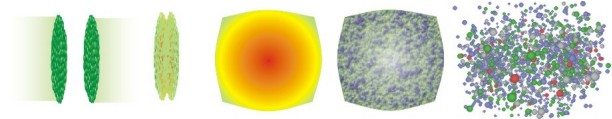
\includegraphics[width=\columnwidth]{pics/evo.jpg}
	\caption{Illustration of multi-stages of a relativistic heavy-ion collision event (Side-view). From left to righ: incoming nuclei, initial state and pre-equilibrium stage, hydrodynamic expansion of QGP, hadronization and hadronic re-scattering. The credit of this figure belongs to Steffen Bass.}
	\label{hybrid}
	\end{center}
	\end{figure}
	\begin{itemize}
		\item Initial conditions. 		
		Initial condition models generate the energy/entropy, baryon density distribution and local flow velocity immediately after the penetration of two nuclei.
		It has been noted that fluctuations in the positions of nucleons are essential to account for higher-order anisotropic flow observed in experiment;
		so, instead of using average nuclear density such as a Wood-Saxon distribution, present simulations use event-by-event nuclear configurations by sampling individual nucleons inside the colliding nuclei.
		
		The system at proper time $\tau = 0$ fm/c should be far from thermal equilibrium; however, in less than $1 \textrm{ fm/c}$, it is believed to be close to local thermal equilibrium.
		The dynamics for this transient pre-equilibrium stage is still not clear.
		So most models such as MC-Glauber, MC-KLN, EKRT, and TRENTo generate initial condition at certain proper time $\tau\sim 0.6 \textrm{ fm/c}$, assuming local thermalization \citep{Miller:2007ri, Drescher:2006ca, Eskola:1999fc, Moreland:2014oya}.
		Other models such as the IP-glasma model \citep{Schenke:2012wb} and free-streaming/sudden thermalize model \citep{Liu:2015nwa} include pre-equilibrium dynamics.
		
		\item Relativistic fluid dynamics. 
		Relativistic viscous hydrodynamics describes the expansion of QGP by solving energy-momentum and charge conservation,
		\begin{eqnarray}
			\partial_\nu T^{\mu\nu} &=& 0, \\
			\partial_\nu N^{\nu} &=& 0,
		\end{eqnarray}
		with an equation of state $p = p(\epsilon, n_B)$ to close the equations. 
		
		Hydrodynamics translates initial state spatial anisotropy into final state momentum-space anisotropy, which is measured in experiments using anisotropic flow observables.
		This can be understood qualitatively from Fig. (\ref{almond}) that an almond shaped blob of thermalized medium has lager pressure gradients in the direction of its short axis than along its long axis, therefore the medium will undergoes a faster expansion in the x-direction than in the y-direction, producing momentum-space anisotropy. 
		\begin{figure}
		\begin{center}
		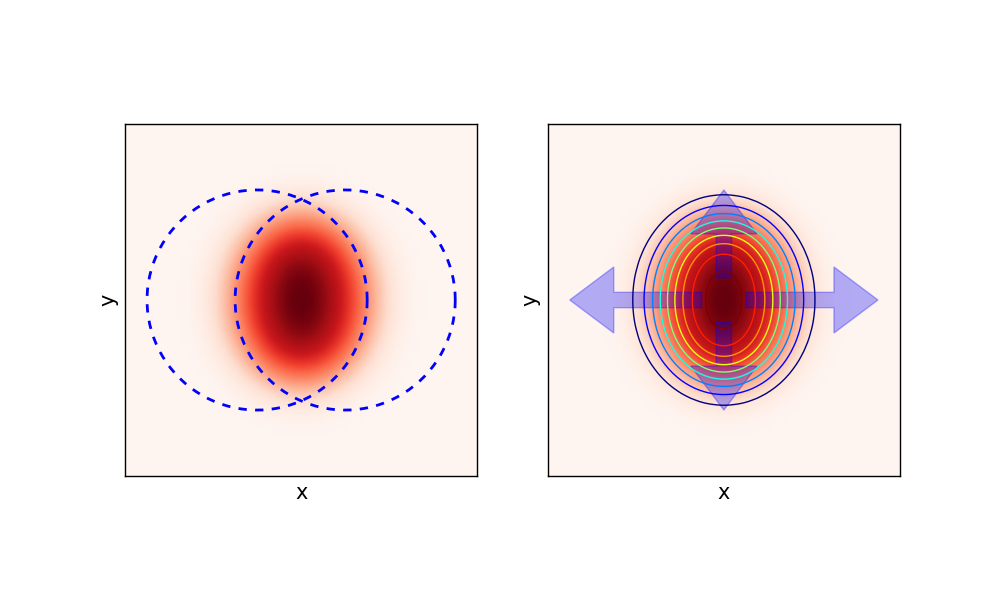
\includegraphics[width=\columnwidth]{pics/almond.png}
		\caption{Left: in the xy plane, two colliding nuclei are denoted by blue dash circle, the deformed red blob in the middle is the deposited energy after the collision to the two nuclei. Right: isobaric contours. System will expand stronger in the short axis direction due to larger pressure gradient.}\label{almond}
		\end{center}
		\end{figure}
		
		Flow observables are sensitive to the transport coefficients such as shear and bulk viscosity in hydrodynamics simulation, which provides tight constraints on the transport properties of QGP.
		
		In the present calculation, 3+1 D relativistic viscous hydrodynamics is employed \citep{Karpenko:2013wva} with a 2+1 flavour QCD equation of state from lattice calculation \cite{Bazavov:2014pvz}.
		

		\item Statistical hadronization. 
		As temperature drops and hydrodynamics ceases to apply, the system is particularized by the statistical sampling of hadrons from particle distribution functions. 
		Under the assumption of sudden hadronization along an isothermal hyper-surface, particles are sampled from the Cooper-Frye formula \citep{Cooper:1974mv},
		\begin{eqnarray}
			E\frac{\mathrm{d}N_i}{\mathrm{d}^3p} = \int_\Sigma f_i(x, p)p^\mu\mathrm{d}^3\sigma_\mu,
		\end{eqnarray}
		where $f_i$ is the phase space distribution of type-``i" particle and $\mathrm{d}^3\sigma_\mu$ is the hyper-surface element.
			
		\item Final state scattering. 
		The system after hadronization is still dense enough to allow hadronic scattering. 
		Transport models such as UrQMD are utilized to solve the Boltzmann equation \citep{Bass:1998ca, Bleicher:1999xi},
		\begin{eqnarray}
			\frac{\mathrm{d}f_i(x, p)}{\mathrm{d}t} = C_i(x, p),
		\end{eqnarray}
	where $C_i$ describes the gain and loss of type-``i" particles due to collisions. 
	\end{itemize}
	


\section{Collision of large / small systems}
The first ultra-relativistic experimental was conducted at RHIC with top energy $\sqrt{s} = 200 \textrm{ GeV/A}$. 
Later, the heavy-ion program at LHC increases this energy to $\sqrt{s} = 2.76 \textrm{ TeV/A}$. 
Apart from a wide range of energies, various systems are examined as well,
\begin{center}
	\begin{tabularx}{0.5\textwidth}{c *{3}{Y}}
	\toprule[1pt]
	System 		& LHC 		 &	RHIC\\
	\midrule[0.5pt]
	Baseline	 	& p + p		 & 	 p + p \\
	\midrule[0.5pt]
	Large and		 	& Pb + Pb	 & 	 Au + Au \\
	symmetric		 	&			 & 	 U + U \\
			 	&			 & 	 Cu + Cu \\
	\midrule[0.5pt]
	Small and 	& p + Pb	 	 & 	 p + Au \\
	asymmetric		 	&			 & 	 d + Au \\
			 	&			 & 	 ${}^3$He + Au \\
	\bottomrule[1pt]
	\end{tabularx}
\end{center}
It was expected that the QGP would be created in large, dense systems (AA collisions) and was not expected to be important in small system such as p+Pb (pA collisions), where cold nuclear matter effects are typically studied.

The observation of azimuthal anisotropy in agreement with hydrodynamic calculations confirms the existence of a strongly coupled QGP phase in large collisions; however, similar phenomena were also observed in small systems p+Pb, p+Au, d+Au and ${}^3$He+Au and even in high multiplicity p+p events at LHC recently  \citep{Loizides:2016tew, Adare:2014keg, Adare:2015ctn, CMS:2015waa, ALICE:2014mda}. These observations suggest that QGP may be produced in small systems as well.

\begin{figure}
\begin{center}
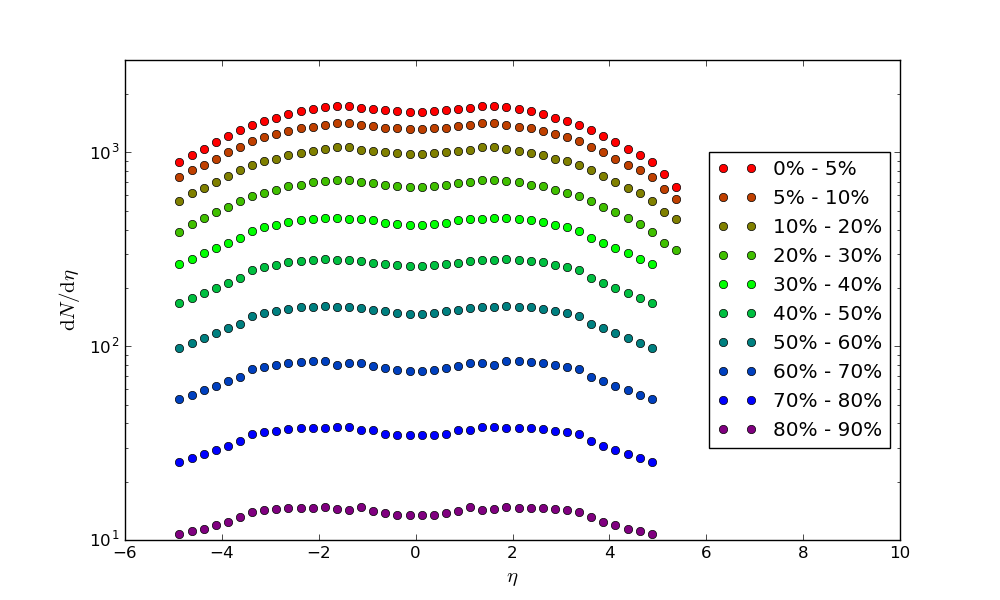
\includegraphics[width=\columnwidth]{pics/dNdy-PbPb.png}
\caption{Centrality dependence of charged particle pseudo-rapidity density in PbPb collision at $\sqrt{s} = 2.76 TeV/A$ from ALICE collaboration \citep{ALICE:2015kda}.}
\label{AA-dNdy}
\end{center}
\end{figure}

\begin{figure}
\begin{center}
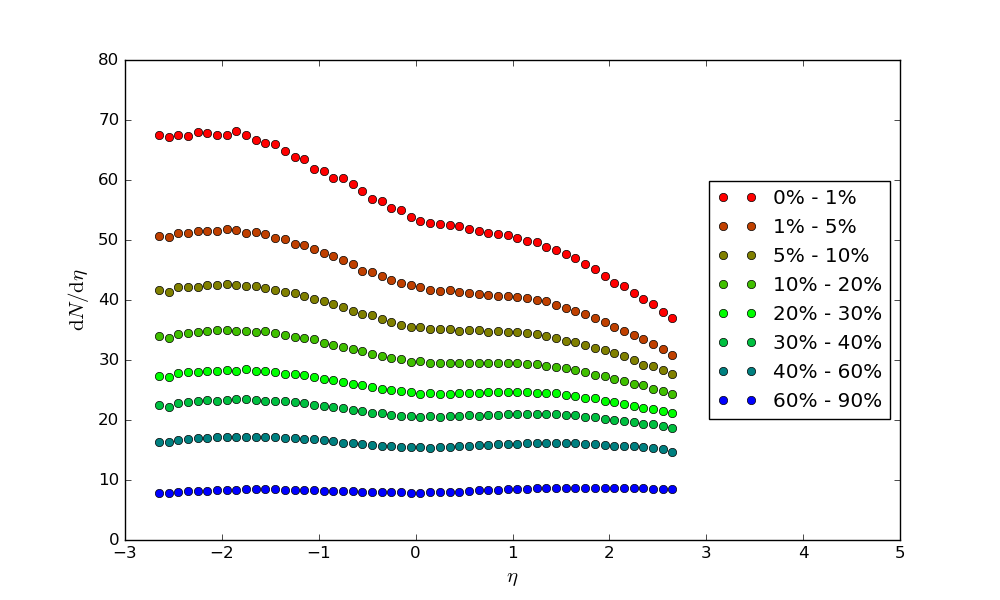
\includegraphics[width=\columnwidth]{pics/dNdy-pPb.png}
\caption{Centrality dependence of charged particle pseudo-rapidity density in pPb collision at $\sqrt{s} = 5.02 TeV/A$ from ATLAS collaboration \citep{Aad:2015zza}.}
\label{pA-dNdy}
\end{center}
\end{figure}

\section{Centrality class, kinetics, and boost-invariance approximation}
	This section will introduce a few useful concepts for describing relativistic heavy-ion collisions.
	
	First we examine the transverse geometry of AA collisions. Collisions at different impact parameters result in different transverse geometries and multiplicities (number of final state charged particles). 
	As seen in Fig. (\ref{centrality}), small impact parameter results in large overlapping between projectile and target nuclei, producing initial condition with small eccentricity and more final state particles; large impact parameter leads to a initial condition with larger eccentricity and less particles in the final state. 
	We are interested in the initial state eccentricities, because they will translate into final state momentum-space anisotropy through hydrodynamics expansion.
	However, experimentally there is no control over the impact parameter, instead the collision geometry is inferred by the event multiplicity or centrality class.
	The definition of centrality class may varies in different experiments.
	For example, if events are sorted according to their multiplicities with certain kinetic cuts in descending order, centrality class $[c_1\%, c_2\%)$ is defined to be the $c_1\%$ to $c_2\%$ of the sorted sequence.
	Therefore, for AA collision, larger centrality class corresponds to smaller multiplicity and smaller initial spatial anisotropy (eccentricity).
	\begin{center}
	\begin{figure}
	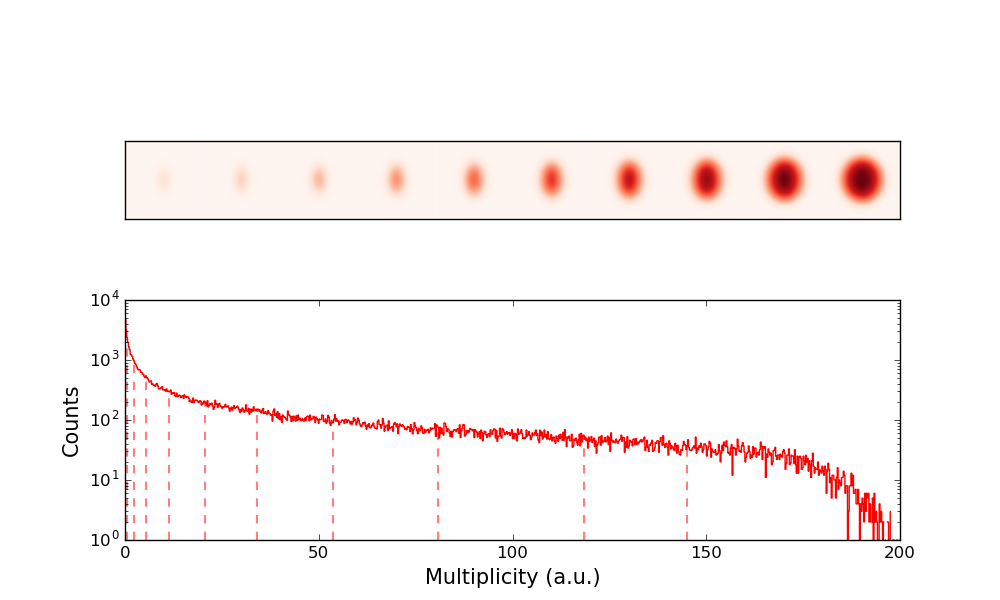
\includegraphics[width=\columnwidth]{pics/centrality.png}
	\caption{Lower: historgram of multiplicity for $10^6$ evnets generated by TRENTo. Vertial dashed lines denotes the range of centrality classes: $0 - 5\%, 5 - 10\%, 10 - 20\%, 20 - 30\%, 30 - 40\%, 40 - 50\%, 50 - 60\%, 60 - 70\%, 70 - 80\%, 80 - 90\%, 90 - 100\%$ from right to left. Upper: typical collision geometry for events within the corresponding centrality class.}\label{centrality}
	\end{figure}
	\end{center}		
	
	Next, we focus on the longitudinal features of the collisions.
	The matter produced in heavy-ion collisions expands rapidly in the beam direction, so it is convenient to use curvilinear coordinates $(\tau, x, y, \eta_s)$. 
	Here $x, y$ are the Cartesian coordinates transverse to the beam direction ($z$ direction), $\tau$ and $\eta_s$ are the local time and space-time rapidity,
	\begin{eqnarray}
		\tau = \sqrt{t^2 - z^2} &,& \eta_s = \frac{1}{2}\ln\left(\frac{t+z}{t-z}\right) \\
		t = \tau \cosh \eta_s &,& z = \tau \sinh \eta_s.
	\end{eqnarray}
	These coordinates transform under lorentz boosts along the $z$ direction as,
	\begin{eqnarray}
		(\tau, {\bf x_{\perp}}, \eta_s) \xrightarrow{L} (\tau, {\bf x_{\perp}}, \eta_s + \Delta)
	\end{eqnarray}
	We also introduce longitudinal rapidity ($y$) and pseudo-rapidity ($\eta$) for momentums of final state particles,
	\begin{eqnarray}
	y &=& \frac{1}{2}\ln\left( \frac{E + p_z}{E - p_z} \right), \\
	\eta &=& \frac{1}{2}\ln\left( \frac{|\vec{p}|+p_z}{|\vec{p}|-p_z} \right) = -\ln\left(\tan\left(\frac{\theta}{2}\right)\right).
	\end{eqnarray}
	The pseudo-rapidity of a particle is directly related to the angle between its momentum and the beam axis, and is therefore convenient for experimental measurements.
	
	A boost-invariant situation refers to a problem set-up without $\eta_s$ dependence, which reduces the 3+1 D hydrodynamic simulation to 2+1 D. 
	A simple case is known as Bjorken flow \citep{Bjorken:1982qr}, where pseudo-rapidity coincides with the space-time rapidity so that medium at space coordinate $z$ recede with a velocity $z/t$ from the center.
	After solving the evolution in the transverse plane at $\eta_s = 0$, the solution at arbitrary $\eta_s$ is obtained by boosting in the beam direction.
	
	Boost-invariance is considered to be a good approximation in AA collisions, as seen from the charged particle pseudo-rapidity distribution measured at RHIC and LHC, Fig. (\ref{AA-dNdy}). 
	Crudely speaking, the central plateau of $\mathrm{d}N/\mathrm{d}\eta$ justifies boost-invariance around $\eta = 0$ since a small shift in $\eta$ makes little difference at $|\eta| < 2$. 
	However, these measurements are performed over many events within each centrality class, so the mid-rapidity plateau may be absent in the evolution of individual events.
	Also, the event-wise longitudinal energy density profile at certain transverse regions may violate boost-invariance, due to local asymmetry of projectile and target densities. 
	How these local longitudinal fluctuations affect our prediction at mid-rapidity and the extraction of transport coefficients should be interesting.
	
	Moreover, from Fig. (\ref{pA-dNdy}), boost-invariance is definitely broken in p+A (asymmetric) collisions.
	Since the observation of collectivity in small systems, there are heated discussion on extending the applicability of hydrodynamics to such systems.
	A consistent comparison of simulation with experimental data requires a more realistic rapidity dependent initial condition as input.
	
	
	
	\section{TRENTo Initial Condition}
	Under the boost-invariance approximation, it is sufficient to specify the initial condition at mid-rapidity ($\eta_s = 0$). Various models were proposed to describe the entropy/energy deposition at mid-rapidity. 
	However, these models can be phenomenologically described with an effective model TRENTo \cite{Moreland:2014oya}. 
	TRENTo IC is constructed in three layers,
	\begin{itemize}
		\item Calculate cross sections using a Glauber formalism.
		\item Determine the density of participant matter. 
		\item Convert local participant density to entropy deposition using a flexible ansatz.
	\end{itemize}
	The first two steps are similar to the procedures of Monte-Carlo Glauber model; however, TRENTo employs a much more generalized entropy deposition formula.
	\subsection{Parametrization of binary nucleon-nucleon collision}
	Impact parameter ($b$) differential inelastic cross-section or the probability of inelastic collision at fixed impacted parameter is calculated in the eikonal limit,
	\begin{eqnarray}\label{dsigma_db}
		\frac{\mathrm{d}\sigma_{NN}}{2\pi b \mathrm{d}b} = 1 - \exp\left(-\alpha T_{pp} (b)\right).
	\end{eqnarray}
Here, $T_{pp}$ is the overlapping of nucleons' transverse density function $\rho(x_\perp)$, which is generally assumed to be normalized Gaussian,
	\begin{eqnarray}
		\rho(x_\perp) &=& \frac{1}{\sqrt{2\pi w^2}}\exp\left(-\frac{{x_\perp}^2}{2w^2}\right), \\
		T_{pp}(b) &=& \int \mathrm{d}{x}^2 \rho(x+\frac{b}{2})\rho(x-\frac{b}{2})
	\end{eqnarray}
	All the information of subnucleonic degrees of freedom is encoded in the coefficient $\alpha$, which is tuned to reproduce the proton-proton inelastic cross section at a given energy,
	\begin{eqnarray}
		\int \mathrm{d}\sigma_{nn}(\alpha) = \sigma_{pp, inel}(\sqrt{s}).
	\end{eqnarray}
	Eq. (\ref{dsigma_db}) is then interpreted as the probability for two nucleons to collide with impact parameter $b$ and is realized via a Monte-Carlo approach.
	\begin{figure}
	\begin{center}
	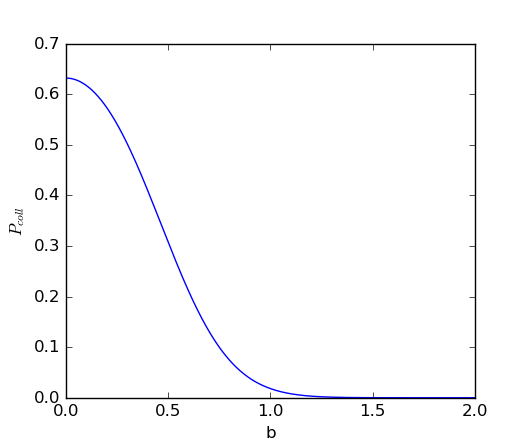
\includegraphics[width=\columnwidth]{pics/Pcoll.png}
	\caption{Impact parameter dependence of nucleon-nucleon inelastic collision probability.}
	\end{center}
	\end{figure}
	\subsection{Determine participant density}
	The time it takes the projectile nucleons to penetrate the target nucleus is much shorter than the time scale of internal motion inside the nucleus; therefore, nucleon position fluctuation cannot be neglect.
	\begin{figure}
	\begin{center}
	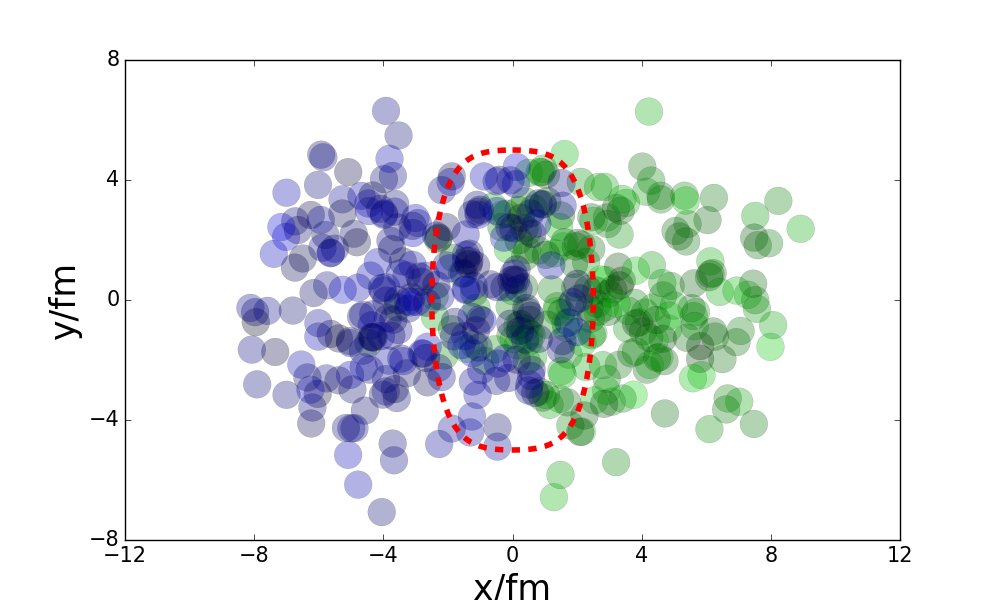
\includegraphics[width=\columnwidth]{pics/nuclei.png}
	\label{nuclei}
	\caption{Transverse view of sampled nucleons from Woods Saxon distribution for target (blue) and projectile (green) nuclei. The impact parameter is $b = 8$ fm. Entropy deposition region is denoted by red dashed circle.}
	\end{center}
	\end{figure}
	
	In TRENTo, nucleons are sampled from a (deformed) Woods-Saxon density distribution and then projected onto the transverse plane. 
	Each pair of nucleons from the projectile and target nuclei are tested with binary collision criterion. 
	Nucleons subject to at least one collision are called participants and the rest spectators.
	The contribution of participants from nuclei $A,B$ defines the nuclear thickness function:
	\begin{eqnarray}
		T_{A,B}(x_\perp) &=& \sum_{i \in \textrm{Part} A,B} \gamma_i \rho(x_\perp- x_i), \\
		\gamma_i &\sim& \Gamma(k, k).
	\end{eqnarray}
	Note that the contribution from each participant nucleon is multiplied by a random variable $\gamma_i$ sampled from a $\Gamma$ distribution with unit mean and variance $1/k$. 
	This additional source of fluctuation is added to reproduce the negative binomial distribution of charged particle multiplicity in minimum bias $pp$ collisions.
	\subsection{Entropy Deposition Ansatz}
	TRENTo assumes in the eikonal limit, immediately after the collision that entropy deposition is a local function of nuclear thickness functions $T_{A,B}$. 
	The generalized mean ansatz provides a flexible way to parametrize this mapping,
	\begin{eqnarray}
	\left.\frac{\mathrm{d^3}s}{\mathrm{d}\eta_s \mathrm{d}x_\perp^2}\right\vert_{\eta_s = 0} &=& 	T_R\left(T_A, T_B; p\right),	\\
	T_R(x, y; p) &=& \left(\frac{x^p+y^p}{2}\right)^{\frac{1}{p}}.
	\end{eqnarray}
	By varying the parameter $p$, the model is able to mimic a variety of initial condition models \cite{Scott}.
	\begin{center}
	\begin{tabularx}{0.45\textwidth}{c>{\centering\arraybackslash}m{2.0cm}>{\centering\arraybackslash}m{2cm} cX}
	\toprule[1pt]
	$p$	&	$-0.67$	 	&	$0.0$ 		& 	$1.0$		\\
	\midrule[0.5pt]	
	$\sim$ &		KLN		& 	EKRT		& 		Wounded Nucleon \\
	\bottomrule[1pt]
	\end{tabularx}
	\end{center}
	The ``$\sim$" sign in the table reminds that $T_R$ resembles the entropy deposition of different models for reasonable value of the participant density. 
	This parametrization allows interpolation between different initial condition models and is suitable for a model selection procedure to learn what is the most probable initial condition to explain the observed experimental data at mid-rapidity.
	A model-to-data comparison using Bayesian analysis constrained the parameter $p$ close to zero \citep{Jonah}.
\section{Rapidity Dependent Extension of TRENTo}
	Although many models have been proposed to describe initial condition at mid-rapidity, it is not clear how to include rapidity dependence. In the same spirit of TRENTo, we choose to parametrize the rapidity dependence of the initial conditions in a flexible and simple way, so that a model selection procedure can be applied.
	
	Because of the success of TRENTo at mid-rapidity, the 3d-extension preserves the prediction of TRENTo at $\eta_s = 0$ and the entropy distribution is still a local function of $T_A$ and $T_B$,
	\begin{eqnarray}
	T_A(x_\perp), T_B(x_\perp) \rightarrow \frac{\mathrm{d^3}s}{\mathrm{d}x_{\perp}^2 \mathrm{d}\eta_s}\left(x_\perp, \eta_s\right)
	\end{eqnarray}
	Also for simplicity, it is assumed the rapidity dependence factorizes from the transverse distribution $T_R$,
	\begin{eqnarray}
		\frac{\mathrm{d}S}{\mathrm{d}x_{\perp}^2 \mathrm{d}\eta_s}  &\propto& T_R(x_\perp) \frac{F(x_\perp,y)}{F(x_\perp,0)}\frac{\mathrm{d}y}{\mathrm{d}\eta_s},
	\end{eqnarray}
assuming the relation between particle's rapidity and space-time rapidity,
	\begin{eqnarray}
		\eta_s &=& \sinh^{-1}(\sqrt{K}\sinh(y)), K>1. 
	\end{eqnarray}
	
	Instead of using any explicit form of the rapidity dependence of $F(x_\perp, y)$, we first parametrize its cumulants and then reconstruct it by applying an inverse Fourier transformation on the cumulant generating function,
	\begin{eqnarray}
	 	F(x_\perp,y) &=& \mathcal{F}^{-1}\{\tilde{F}(k)\} \\
	 	\ln \tilde{F} &=&  i \mu k - \frac{1}{2}\sigma^2 k^2 + i 	\gamma k^3  - \kappa k^4 ...
	\end{eqnarray}

	Different rapidity dependent IC models can be mapped to different parametrization of cumulants. Two existing approaches with the name ``Shifted" or ``Tilted" are listed in the first two rows \cite{Bozek:2010bi}.
	\begin{widetext}
	\begin{center}
	\begin{tabularx}{0.8\textwidth}{c *{4}{Y}}
	\toprule[1pt]
	Cumulants & mean &	std	& skewness	& kurtosis \\
	\cmidrule[0.5pt]{2-5}
		&	$\mu(x_\perp)$ & $\sigma(x_\perp)$& $\gamma(x_\perp)$  & $\kappa(x_\perp)$	\\
	\midrule[0.5pt]
	shifted & $\frac{1}{2}\ln\frac{T_A}{T_B}$ & const. &  $0$	&const.\\
	tilted & $0$ & const.& $T_A - T_B, \frac{T_A-T_B}{T_A+T_B}$	& const.\\
	general & $\frac{a}{2}\ln\frac{T_A}{T_B}$& b  & $c(T_A - T_B)$ & d \\
	\bottomrule[1pt]
	\end{tabularx}
	\end{center}
	\end{widetext}
	A shifted initial condition assumes that in asymmetric collisions, particle production (local in transverse plane) as function of rapidity resembles a Gaussian in the symmetric case, with its mean shifted to the center-of-mass rapidity $\frac{1}{2}\ln(T_A/T_B)$. 
	A tilted initial condition modifies the symmetric distribution by a linear tilting,
	\begin{eqnarray}
	f_{\textrm{asy}}(\eta_s) = f_{\textrm{sym}}(\eta_s) (1+\alpha \eta_s)
	\end{eqnarray}
	where $\alpha$ is a measure of the degree of asymmetry. 
	Two possible constructions for the degree of asymmetry are shown in the second row. 
	This first one is a dimensionfull quantity while the second is a dimensionless construction. 
	In the last row, we show a general case with the mean proportional to the center-of-mass rapidity and the skewness proportional to the degree of asymmetry. 
	By varying the coefficients $a, c$, we are able to interpolate between these two entropy deposition schemes.
	
	\begin{figure}
	\begin{center}
	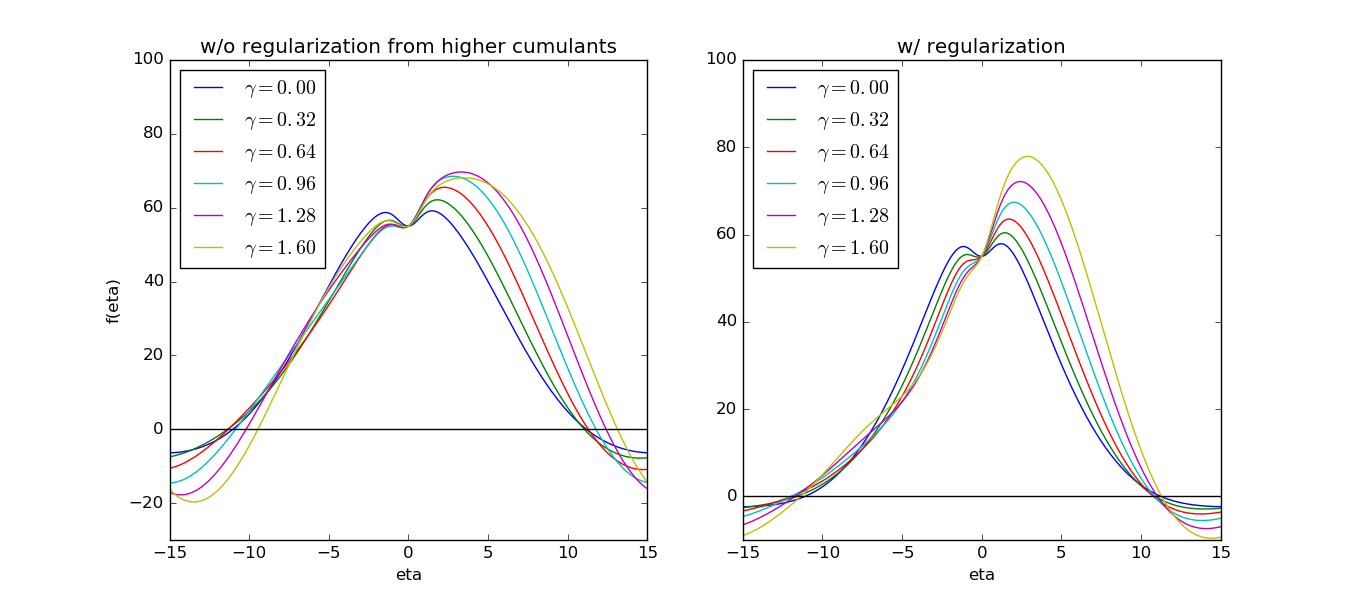
\includegraphics[width=\columnwidth]{pics/regulate.png}
	\caption{Left: parametrized longitudinal entropy deposition for different values of the skewness $\gamma$ suffers from non-monotonic behaviour as function of skewness at central rapidity and negative values at large rapidity. Right: replacing $\gamma$ by $\gamma\exp{\left(-\frac{1}{2}\sigma^2 k^2\right)}$ achieves desired monotonic change with skewness and suppresses negative regions at large rapidity.}\label{regulation}
	\end{center}
	\end{figure}
 
	However, the reconstructed function may not be well-behaved for relatively large skewness. 
	From the left panel of Fig. (\ref{regulation}), with the increase of skewness, there is not a monotonic trend of change; also, the function goes negative for large $|\eta_s|$.
	This stresses the importance of including higher order cumulants to regularize the behaviour of the generating function. 
	The conditions to ensure a positive definite Fourier transform are quite involved, but with the following substitution,
	\begin{eqnarray}
		\{\gamma, \kappa\} \rightarrow \{\gamma, \kappa\} \exp\left(-\frac{1}{2}\sigma^2k^2\right),
	\end{eqnarray}
	the negative region is suppressed and there is a clear monotonic trend with increasing skewness in Fig. (\ref{regulation}). The range of skewness shown in the plot covers the largest reasonable values for realistic initial conditions.	
	Note that this substitution leaves the skewness and kurtosis intact, while contributions from higher order cumulants are included systematically.
	The distribution reconstructed with regularization is positive and well behaved over a wide range of rapidity and skewness.
	
	Fig. (\ref{3d-example}) shows a sample 3d initial condition event for PbPb and pPb collisions, projected onto the X-Y plane at mid-rapidity, to the X-$\eta_s$ plane at $Y = 0$ and to the Y-$\eta_s$ plane at $X = 0$. We can see that the transverse entropy distribution fluctuates due to randomized nucleon positions, and the longitudinal profile is distorted forward/backward according to the asymmetry of local target and projectile densities. 
	
	\begin{figure}
	\begin{center}
	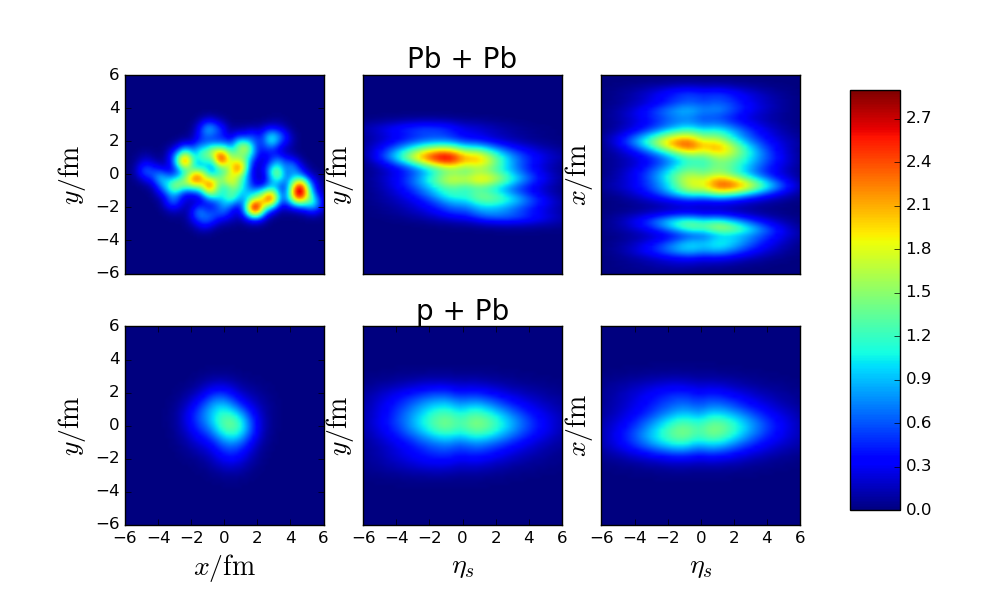
\includegraphics[width=1.0\columnwidth]{pics/3d-example.png}
	\caption{Upper: IC of a PbPb event projected onto XY, YZ, XY plane (from left to right). Lower: IC of a pPb event projected onto XY, YZ, XY plane (from left to right).}\label{3d-example}
	\end{center}
	\end{figure}
	

\section{Model to Data Comparison}
	The ultimate goal is to compare the calculations of hybrid models with different initial conditions to experimental measurements. This improves our knowledge of initial conditions and other model parameters such as transport coefficients. We briefly summarize the procedures for model-to-data comparison using Bayesian analysis \citep{Dave:10.2307/27640080, Bernhard:2015hxa}. 
	\subsection{Parameter design} 
	Hybrid models for heavy-ion physics usually contain multiple parameters. 
	A 3d extension of the existing initial condition introduces $4\sim5$ additional parameters.
	This constitutes a high dimensional parameter space $(p_1, p_2, ..., p_d)$, which is impractical for uniform search. 
	A Latin hypercube experimental design is preferable for this problem. 
	In such an experimental design, parameters (properly normalized to live in $[0,1)^d$) are generated using a Monte Carlo approach, such that
	\begin{itemize}
		\item The minimum distance between parameter points is maximized.
		\item The projection of sampled parameter points onto lower dimensional space is uniformly distributed.
	\end{itemize}
	The advantage of Latin hypercube design is that it avoids over populated or sparse regions of parameter space and that the number of samples needed scales linear with the dimension of the parameter space.
	
	The parameter set and its range in the present 3d initial condition is,
	\begin{center}
	\begin{tabularx}{0.45\textwidth}{c*{7}{Y}}
		\toprule[1pt]
		 & Norm	& fluct	& $a$ & $b$ & $c$ & $d$ & $K$ \\
		\midrule[0.5pt]
		lower & $8.$		&  $1.$	&	$0.$&	 $2.$ & $0.$ & $0.2$ & $0.6$ \\
		upper	& $12.$		&  $4.$	&	$2.$& $4.$ & $0.5$ & $0.8$ & $0.8$ \\
		\bottomrule[1pt]
	\end{tabularx}\label{parameter}
	\end{center}
	The model runs on the $N$ sets of sampled parameters and then outputs $m$ observables. Loosely speaking, the model maps the design matrix $(N \times d)$ to observable matrix $(N \times m)$,
	\begin{eqnarray}\label{design-obs}
	\left(\begin{array}{ccc}
	p_{1}^{1}  & \cdots & p_{d}^{1}\\
	\vdots  & \ddots & \vdots\\
	p_{1}^{N}  & \cdots & p_{d}^{N}\\
	\end{array}\right)
	\xrightarrow{\textrm{Model}} 
	\left(\begin{array}{ccc}
	O_{1}^{1}  & \cdots & O_{m}^{1}\\
	\vdots  & \ddots & \vdots\\
	O_{1}^{N}  & \cdots & O_{m}^{N}\\
	\end{array}\right)
	\end{eqnarray}
	
	\subsection{Model emulator}
	Model calculations are inferred at arbitrary points in parameter space using a Gaussian process (GP) emulator to interpolate the Latin hypercube design. 
	GP emulator is a powerful non-parametric, non-linear multivariate regression. 
	It predicts the likelihood of model outputs at desired point in parameter space by specifying its mean and the covariance.
	These features make it a flexible tool for inference of model output with uncertainty estimation.
	
	 The Gaussian process is trained and optimized with mapping (\ref{design-obs}), and then serves as a fast surrogate to infer model calculation with a given parameter set $p^*$,
	 \begin{eqnarray}
	 	(p^*_1, \cdots, p^*_d) \xrightarrow{\textrm{trained GP}} (O^*_1, \cdots, O^*_m).
	 \end{eqnarray}
	 
	 \begin{itemize}
	 \item {\bf Gaussian process of d-dimensional scalar function}
	 
	 Given an array of input d-vectors $\{\mathbf{x}_i, i = 1, 2, \cdots, N\}$, Gaussian process is the multivariate normal distribution of the scalar outputs $\{y_i, i = 1, 2, \cdots, N\}$,  with specified mean and covariance matrix,
	 \begin{eqnarray}
	 y_i \sim \mathcal{N}(\mu_i, \Sigma_{ij}).
	 \end{eqnarray}
An instantiation of $y_i$ can be regarded as $N$ points $(\mathbf{x}_i, y_i)$ drawn from a random function with its properties described by $\mu(\mathbf{x}), \Sigma(\mathbf{x}, \mathbf{x}')$.  
	The mean $\mu(\mathbf{x})$ is often set to zero without loss of generality and a common parametrization of $\Sigma(\mathbf{x}, \mathbf{x}')$ is:
	\begin{eqnarray}\label{kernel}
		\Sigma(\mathbf{x}, \mathbf{x}') &=& \sigma_0^2\exp\left( -\frac{1}{2}\Delta\mathbf{x}^T \mathbf{C} \Delta\mathbf{x} \right) + \sigma_n^2\delta_{\mathbf{x}, \mathbf{x}'}, \\
		\Delta\mathbf{x} &=& \mathbf{x} - \mathbf{x}'	
	\end{eqnarray}
	With  matrix $C$ often in diagonal form,
	\begin{eqnarray}
		\mathbf{C} = 
		\left(		
		\begin{array}{cccc}
			l_1^{-2} 	& 	0 		&	 \cdots & 0	\\
			0 			& l_2^{-2}	 & 		\cdots & 0	\\
			\vdots 			& \vdots & \ddots & \vdots	\\
			0 			& 		0 & \cdots & l_d^{-2} \\
		\end{array}
		\right)
	\end{eqnarray}
	Therefore, the variance of $y(\mathbf{x})$ is $\sigma_n^2$ and nearby $\mathbf{x}$'s are mapped to similar $y$'s, while large separations $| \Delta \mathbf{x} | \gg l$ result in almost uncorrelated outputs.
	 
	 
	 \item {\bf Constrained Gaussian process:}
	 GP emulator needs to be constrained to agree with the existing data before it is used for model inference.
	 The constrained GP predicts $y(\mathbf{x}^*)$ (with zero mean) according to,\begin{widetext}
	 \begin{eqnarray}
	 	y(\mathbf{x}^*) &\sim& \mathcal{N}\left(0, \Sigma^*\right), 
	 	\phantom{123}
	 	\Sigma^* = \Sigma(\mathbf{x}^*, \mathbf{x}_i) -  \Sigma(\mathbf{x}^*, \mathbf{x}_i) \Sigma(\mathbf{x}_i, \mathbf{x}_j)^{-1} \Sigma(\mathbf{x}_j, \mathbf{x}^*).
	 \end{eqnarray}
\end{widetext}
	 This guarantees that the closer $\mathbf{x}^*$ is to a data point $\mathbf{x_i}$, the output predicted by GP is closer to $y_i$ due to the reduced covariance. 
	 On the other hand, the uncertainty will be large for prediction of the model output at a value of $\mathbf{x}^*$ far from existing data.

	\item{\bf Training Gaussian process}
	A Gaussian process also introduce its own parameters, or hyper-parameters, such as $\{\sigma_n, l_i, \sigma_0\}$ in Eq. (\ref{kernel}) denoted by $\theta$. In principle, our lack of knowledge of the values of hyper-parameters should be another source of ignorance in addition to the unconstrained model parameters. However, it is common to use an approximation where hyper-parameters are chosen to maximize the model likelihood function \citep{GP-book},
	\begin{eqnarray}
		\ln P(y_i|\mathbf{x}_i, \theta) = -\frac{1}{2}y_i (\Sigma_y^*)^{-1}_{ij} y_j - \frac{1}{2}\ln|\Sigma_y^*| + C,
	\end{eqnarray}
	where $\Sigma_y^*$ is the constrained covariance matrix applied on data points and $C$ is a normalization constant. The first term favours fitting existing data, while the second term is a complexity penalty term that limits over fitting.
	
	\item{\bf Multivariate output}
	The Gaussian process described above only predicts a scalar function, however, model outputs could be high dimensional. 
	Naively, we can construct $m$ Gaussian processes for each column in mapping (\ref{design-obs}), however, it is redundant for strongly correlated observables and also impractical when $m$ is large. 
	Instead, the data dimension is first reduced by principal component analysis. A singular value decomposition (SVD) is performed on the observable matrix in mapping (\ref{design-obs}) and the outputs are rotated to principle components. 
	The relevant principle components that will be emulated by GP are those correspond to the first few largest singular values. 
	They are responsible for most of the modulation of the model outputs. Therefore, by emulating just a few principle components, it captures the main features of the model. 
	Of course, model output can be recovered by transforming back the truncated principle component vector.
	\end{itemize}
	
	\subsection{Model calibration / selection}
	Usually, there is a probability distribution of model parameters even before comparing  to experiment, called priori probability distribution $P(\mathbf(x)^*)$. 
	This priori distribution encodes our existing knowledge of the model, which is often a uniform distribution within a d-dimensional hypercube. 
	By performing a model-to-data comparison, the improved probability distribution of the ``true" values of parameters, called posterior probability distribution, is given by Bayes' theorem,
	\begin{eqnarray}
		P(x^*|\{\mathbf{x}_i, y_i\}, y_\textrm{exp}) \propto P(y_\textrm{exp}|\{\mathbf{x}_i, y_i\}, x^*) P(x^*).
	\end{eqnarray}
	It states that probability of model parameters with given training data sets $\{\mathbf{x}_i, y_i\}$ and experiment, equals the prior probability times the probability of predicting experimental data with given training data sets and model parameters.
	We assume a Gaussian form of $P(y_\textrm{exp}|\{\mathbf{x}_i, y_i\}, x^*)$,
	\begin{eqnarray}
	\ln P(y_\textrm{exp}|x^*) \sim -\frac{1}{2}(y^* - y_\textrm{exp})^T\Sigma_y^{-1}(y^* - y_\textrm{exp})
	\end{eqnarray}
	
	The full posterior is a d-dimensional multi-variate distribution, which can be sampled from the Markov chain Monte Carlo (MCMC) procedure. 
	Information such as marginal probability distribution and correlations between parameters can be extracted from the resulting MCMC ensemble of parameters.
	
\section{Results}
	\subsection{IC against experiment}
	Compared to the boost-invariant 2+1 d case, 3+1 d hydrodynamics is computationally intense for mid-central to central AA collisions. 
	As a result, before performing statistical analysis on the full time evolution, it is advantageous to first compare IC prediction directly against observables that are not very sensitive to dynamics. 
	The charged particle pseudo-rapidity distribution very well serves this purpose, since it approximately scales with initial entropy density.
	It is hoped that this comparison will provide a crude constraint on the IC model.
	
	We sampled 100 parameter sets from the uniform distribution described preciously.
	1000 Pb+Pb events and 1000 p+Pb events were generated for each set.  
	Events are then binned into 10(8) centrality class for Pb+Pb (p+Pb) according to the entropy density at mid-rapidity for Pb+Pb and backward rapidity (Pb going side) for p+Pb to mimic the experimental centrality selection.
	The concatenation of $\mathrm{d}S/\mathrm{d}\eta_s$ of all centralities forms the output vector of the model with one set of parameter inputs. 
	The 100 output vector forms the observable matrix, while parameter vectors forms the design matrix. 
	A principal value decomposition is performed on the observable matrix and the first 5 principal components, covering over 99.5$\%$ variance of the data, are used to describe the model output. 
	The cumulative variance is displayed in Fig. (\ref{weight}).
	
	\begin{figure}
	\begin{center}
	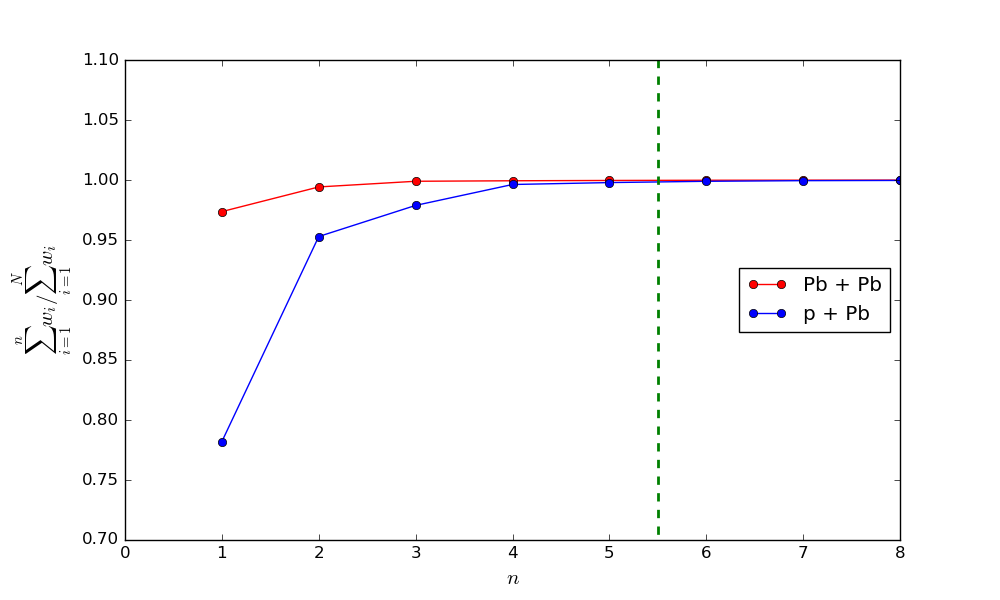
\includegraphics[width=\columnwidth]{pics/weight.png}
	\caption{Fraction of model output variance covered by the first $n$ principal components. The model output for PbPb and pPb were reduced to the first 5 principal components in our calculation, accounting for over 99.5\% of the data.}\label{weight}
	\end{center}
	\end{figure}
	
	Each of the 5 mappings from parameter space to principal components is emulated by an independent Gaussian process.
	The hyper-parameters of the Gaussian process are optimized to maximize the model likelihood.
	Finally using a MCMC procedure, the high dimensional posterior distribution is obtained as an ensemble of equilibrated parameter sets.
	
	It should be noted that measurements of p+Pb and Pb+Pb are conducted at different energies ($\sqrt{s}$ = 5.02 TeV/A and 2.76/A TeV respectively). 
	Because phenomenological parameters generally change with $\sqrt{s}$, it is not fully consistent to compare the model to a combined set of experimental observables at different energies.
	Of course we may assume that the parameters do not change drastically by increasing $\sqrt{s}$ from 2.76 TeV/A to 5.02 TeV/A since they are much higher than other interested scales.
	But for consistency, we run two model-to-data comparisons for p+Pb and Pb+Pb systems separately.
	With the future availability of p+Pb and Pb+Pb data at the same energy, a constraint combining measurements of the two systems is possible.
	
	Here we present the priori and posterior distributions of the observable $\mathrm{d}S/\mathrm{d}\eta_s$ in Fig. (\ref{pri-post-PbPb}) and (\ref{pri-post-pPb}).
	The green dots are points extracted from experimental measurements. 
	Blue thin lines characterise the model output distribution with little knowledge of the true value of parameters (priori distribution); while red lines are output after model-to-data constraint (posterior distribution).
	The results show that the charged particle pseudo-rapidity distribution can be very well reproduced by our general formula for asymmetric entropy deposition.
	Of course, the present result only works under the assumption that final state charged particle multiplicity is proportional to initial entropy. 
	In the full evolution model, viscous effects during hydrodynamic evolution and inelastic scattering processes after freeze-out may slightly change this relation.
	
	\begin{figure}
	\begin{center}
	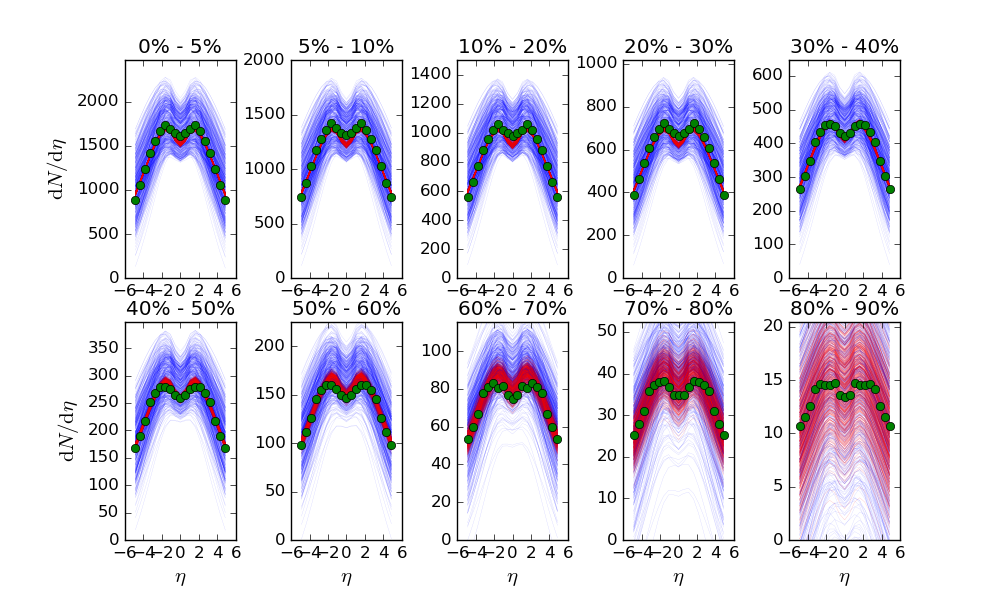
\includegraphics[width=\columnwidth]{pics/pri-post-PbPb.png}
	\caption{Priori / posterior distribution of $\mathrm{d}N/\mathrm{d}\eta$ compared to PbPb data at $\sqrt{s} = 2.76$ TeV. The ensemble of blue thin lines and red thin lines characterize the priori and posterior distribution of $\mathrm{d}N/\mathrm{d}\eta$ respectively, while experimental data are denoted by green dots.}\label{pri-post-PbPb}
	\end{center}
	\end{figure}
	
	\begin{figure}
	\begin{center}
	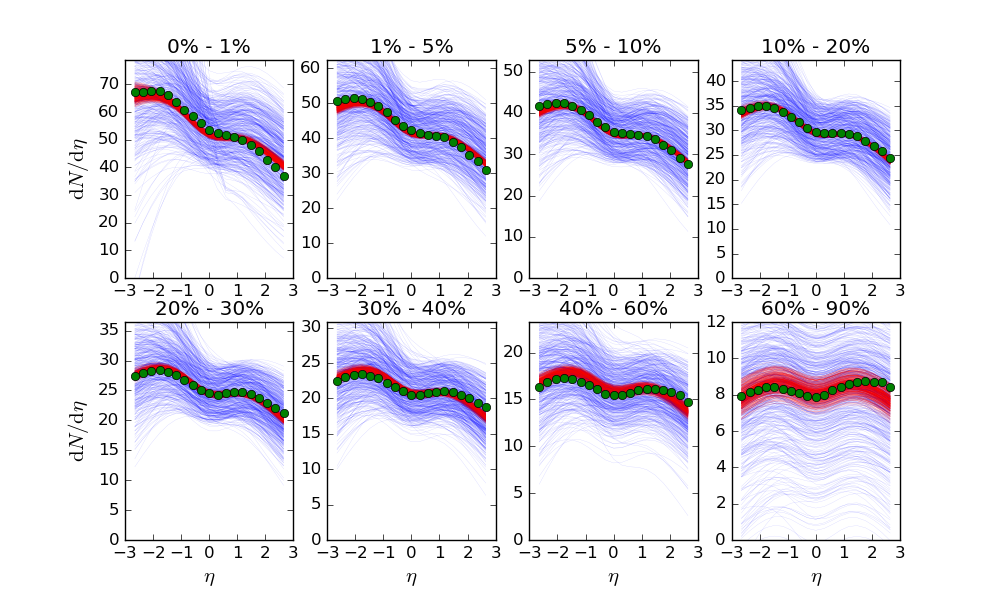
\includegraphics[width=\columnwidth]{pics/pri-post-pPb.png}
	\caption{Priori / posterior distribution of $\mathrm{d}N/\mathrm{d}\eta$ compared to pPb data at $\sqrt{s} = 2.76$ TeV. The ensemble of blue thin lines and red thin lines characterize the priori and posterior distribution of $\mathrm{d}N/\mathrm{d}\eta$ respectively, while experimental data are denoted by green dots.}\label{pri-post-pPb}
	\end{center}
	\end{figure}
	 
	To examine to how well the phenomenological parameters are constrained by experiment, we marginalize the posterior distribution of model parameters. 
	In Fig. (\ref{corner-PbPb}) and (\ref{corner-pPb}) we present the corner plots of the posterior distribution. 
	Diagonal blocks are the marginalized distribution on individual parameters, while the off-diagonal blocks show the correlation between two parameters. 
	Here are some important observations:
	\begin{itemize}
	\item PbPb data does not constrain the fluctuation $k$ very well; but pPb data is much more sensitive and yields a distribution of $k$ peaked around 3.
	\item pPb analysis favours a relatively large Jacobi factor and PbPb the opposite. 
	This and the previous observation indicate that a combined analysis on both systems will benefit from the complementary constraint power of the two systems.
	\item The marginalized posterior for the standard deviation ($\sigma$) of initial entropy longitudinal distribution favours a larger value in p+Pb than that in Pb+Pb analysis. 
	This difference is expected since collision at higher energies should result in a broader pseudo-rapidity distribution. 
	\item  An interesting result is that the mean coefficient is peaked around 1, indicating the mean rapidity of the asymmetrically produced matter is close to the center-of-mass rapidity of local target and projectile densities.
	\end{itemize}
	
	\begin{figure}
	\begin{center}
	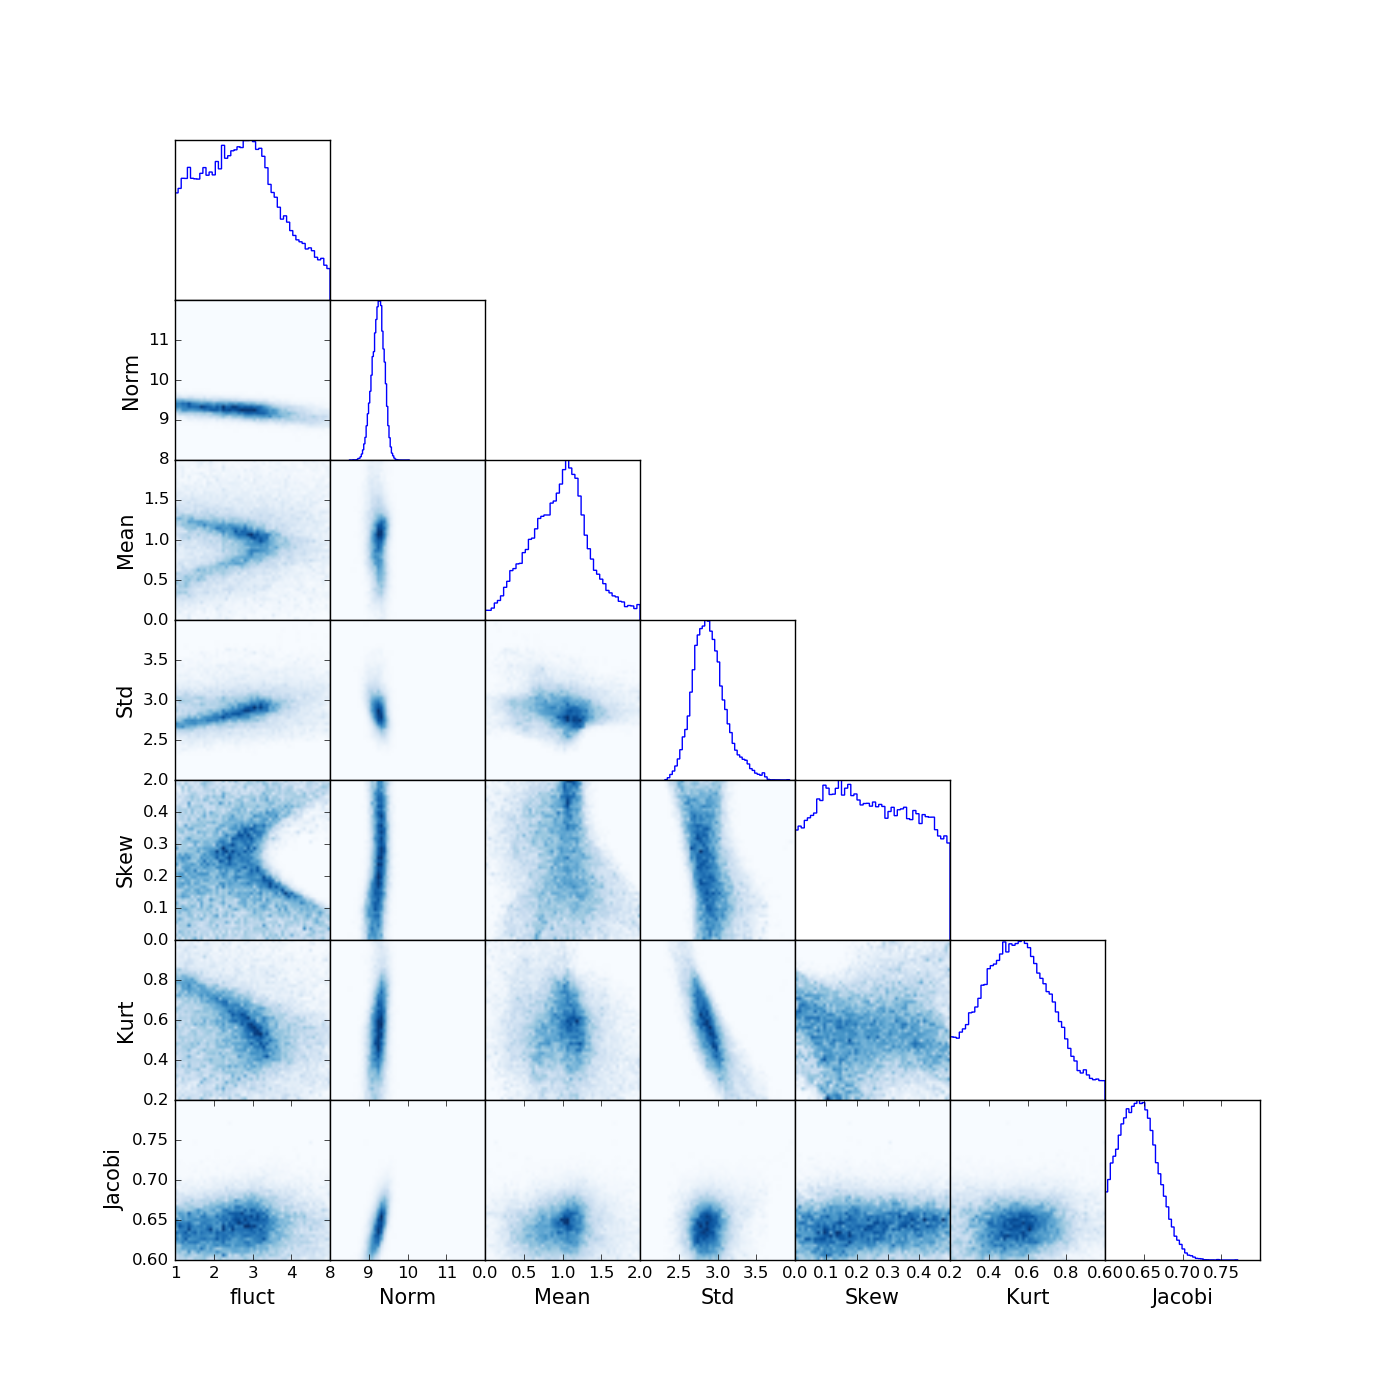
\includegraphics[width=\columnwidth]{pics/corner-PbPb.png}
	\caption{Marginalized posterior distribution of the parameters using PbPb data at $\sqrt{s} = 2.76$ TeV. The diagonal blocks are the marginalized posterior probability distributions of individual parameters; off-diagonal blocks are the marginalized associate distributions of two parameters.}\label{corner-PbPb}
	\end{center}
	\end{figure}
	
	\begin{figure}
	\begin{center}
	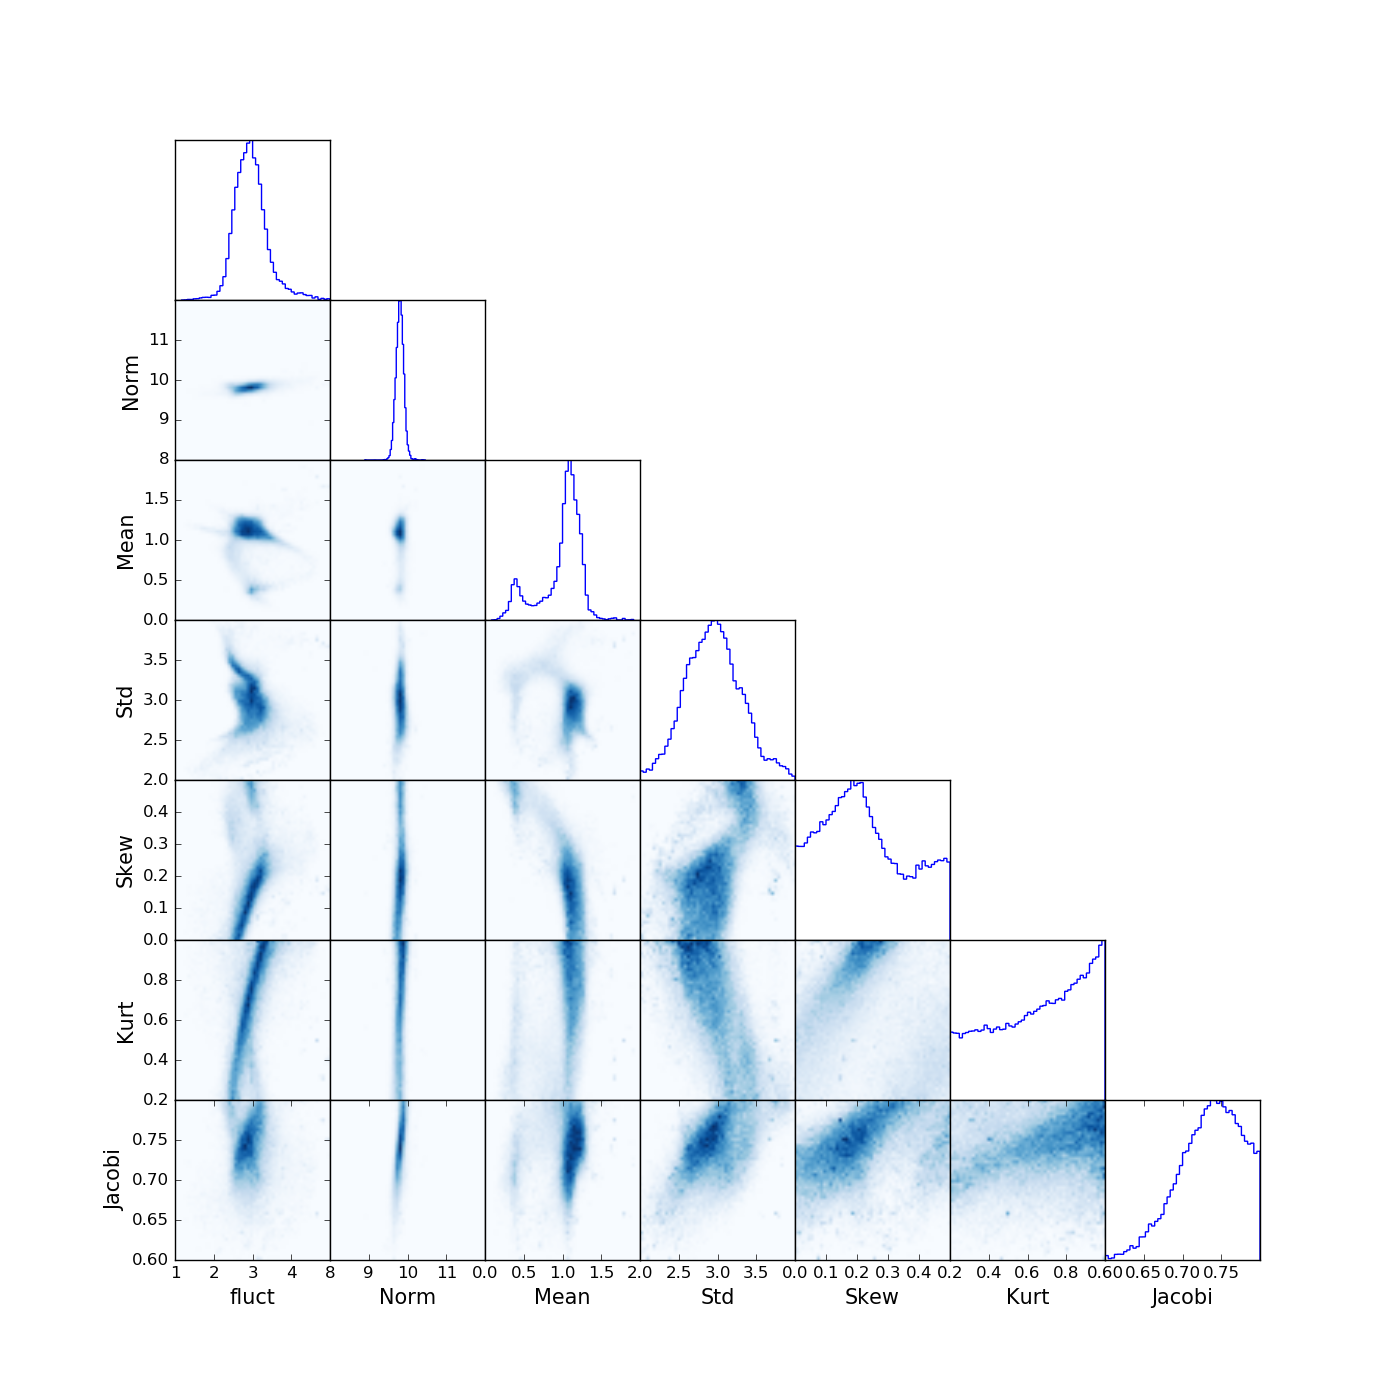
\includegraphics[width=\columnwidth]{pics/corner-pPb.png}
	\caption{Marginalized posterior distribution of the parameters using pPb data at $\sqrt{s} = 5.02$ TeV. The diagonal blocks are the marginalized posterior probability distributions of individual parameters; off-diagonal blocks are the marginalized associate distributions of two parameters.}\label{corner-pPb}
	\end{center}
	\end{figure}	
	
	\subsection{Full time evolution and observables}
	We take a set of parameters around the maximum of posterior distribution and run it through the hydrodynamics evolution and the hadronic phase. 
	The switching temperature $T_s = 0.148 \textrm{ GeV}$ from hydrodynamic to Boltzmann transport description is chosen slightly below the pseudo-critical temperature of the equation of state $T_c = 0.154 \textrm{ GeV}$. The transport coefficients are taken as follows:
	\begin{eqnarray}
		\frac{\eta}{s}  & = & 
		\left\{ \begin{array}{l}
		0.08 + 0.13 \frac{T - T_c}{T_c} \phantom{0.8} , T > T_c \\
		0.8 \phantom{0.12 + 0.13 \frac{T - T_c}{T_c}}, T < T_c
		\end{array}
		\right.	\\
		\frac{\zeta}{s} &=&  0.
	\end{eqnarray}
	Thus, there is no bulk viscosity for simplicity and the shear viscosity over entropy ratio parametrisation has a minimum at $T_c$ and slowly increases with temperature linearly in the QGP phase, while it remains constant in the hadronic phase.
		
	The output of the full time evolution is a list of particles with their final state momentum and type information.
	Apart from charged particle pseudo-rapidity density, more soft observables can be extracted as listed here,
	\begin{itemize}
	\item Transverse energy pseudo-rapidity distribution.
	\item Identified particle transverse momentum spectra.
	\item Particle ratios.
	\item Directed flows, which may be sensitive to different schemes of initial longitudinal entropy deposition according to \citep{Bozek:2009ty}.
	\item Anisotropic flows, including $p_\textrm{T}$ integrated / differential flows, correlation between different flow harmonics and event-by-event flow distributions. Recently as pointed out in \citep{Denicol:2015bnf}, anisotropic flow as function of rapidity is sensitive to the temperature dependence of $\eta/s$. We would like to examine how stable they are against the uncertainties of 3d initial conditions.
	\item Event plane decorrelation and twisting effects \citep{CMS:2015oea}.
	\item Forward backward asymmetry and $\mathrm{d}N /\mathrm{d}\eta$ longitudinal fluctuation.
	\end{itemize}
	
	For the moment, we focus on the charged particle pseudo-rapidity distribution, $p_T$ integrated flow at mid-rapidity and flow as a function of pseudo-rapidity only. 
	Flow coefficients are calculated using the cumulant method described in \citep{Bilandzic:2010jr} with the same kinetic cuts as experimental measurements.
	
	Fig. (\ref{PbPb-dNdy-calc}) and  (\ref{pPb-dNdy-calc}) shows the charged particle distribution after full time evolution. 
	It agrees very well with the experimental measurement over a wide range of centrality classes. 
	Fig. (\ref{PbPb-vn-calc}) shows integrated flow as a function of centrality. 
	Second, third and fourth order flow harmonics $v_2\{2\}$, $v_3\{2\}$ and $v_4\{2\}$ are calculated from two particle correlation. Second order flow from four particle correlation $v_2\{4\}$ is also shown for comparison.
	The $\eta$ dependence of $v_2\{2\}$ is shown in Fig. (\ref{PbPb-vn-eta-calc}). The results show a weak pseudo-rapidity dependence of $v_2\{2\}$, as is suggest by ATLAS measurements \citep{ATLAS:2014eoa}.
	We also calculated directed flow as shown in Fig. (\ref{RUN-1-PbPb-v1-eta}). 
	However, ALICE measures directed flow by correlating particles emitted from the QGP with the spectators' distribution.
	But spectator information is omitted in the present calculation, so we just present $\langle\langle \mathbf{p}_T\cdot \hat{b}/p_T\rangle\rangle$ to estimate the magnitude of directed flow and check if our calculation works qualitatively.
	Our result show a linear $v_1-\eta$ relation with negative slope and weak centrality dependence.
	These qualitative features agree with ALICE measurement \citep{Abelev:2013cva}.
	\begin{figure}
  	\centering
	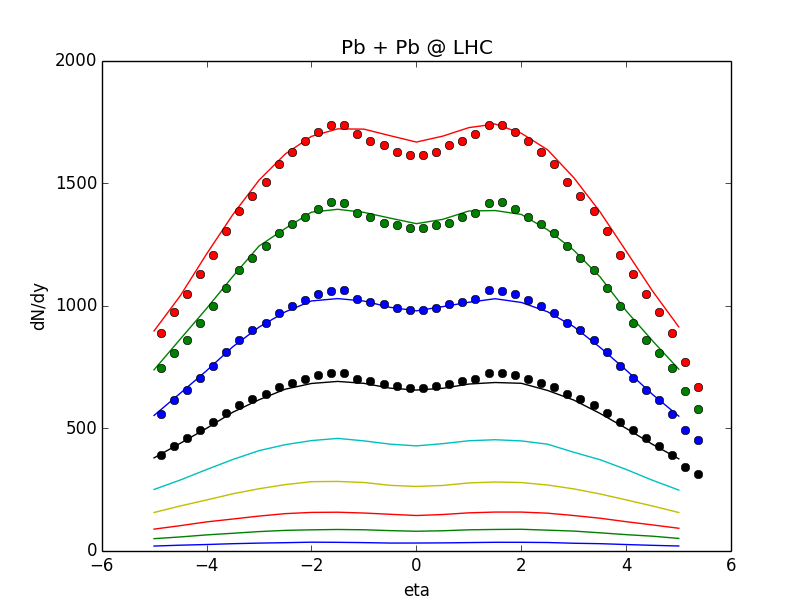
\includegraphics[width=\columnwidth]{pics/RUN-1-PbPb-dNdy-eta.png}
  	\caption{Centrality dependence of $\mathrm{d}N/\mathrm{d}\eta$ of PbPb at $\sqrt{s} = 2.76$ TeV from hybrid model compared to experimental data.}
  	\label{PbPb-dNdy-calc}
	\end{figure}
	
	\begin{figure}
  	\centering
	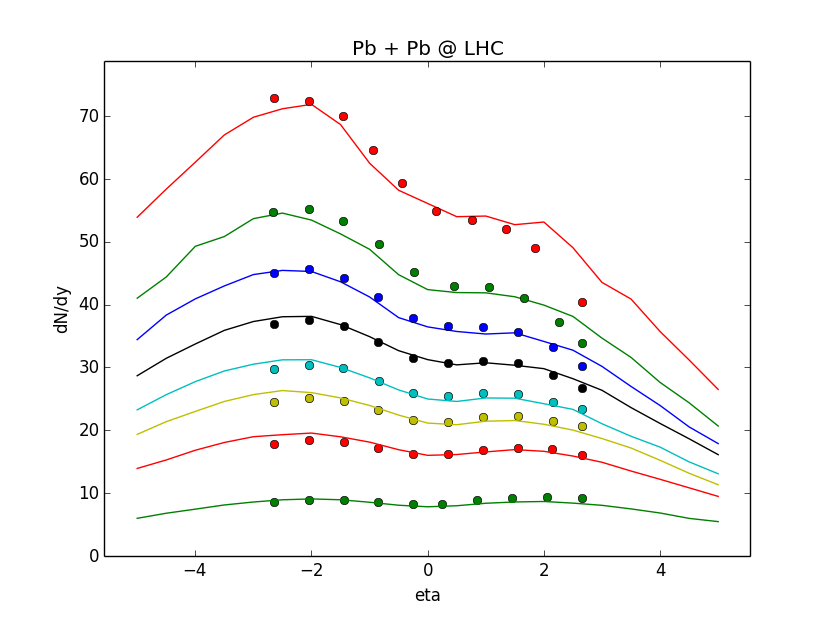
\includegraphics[width=\columnwidth]{pics/RUN-1-pPb-dNdy-eta.png}
	\caption{Centrality dependence of $\mathrm{d}N/\mathrm{d}\eta$ of pPb at $\sqrt{s} = 5.02$ TeV from hybrid model compared to experimental data.}
  	\label{pPb-dNdy-calc}
	\end{figure}
	
	\begin{figure}
  	\centering
	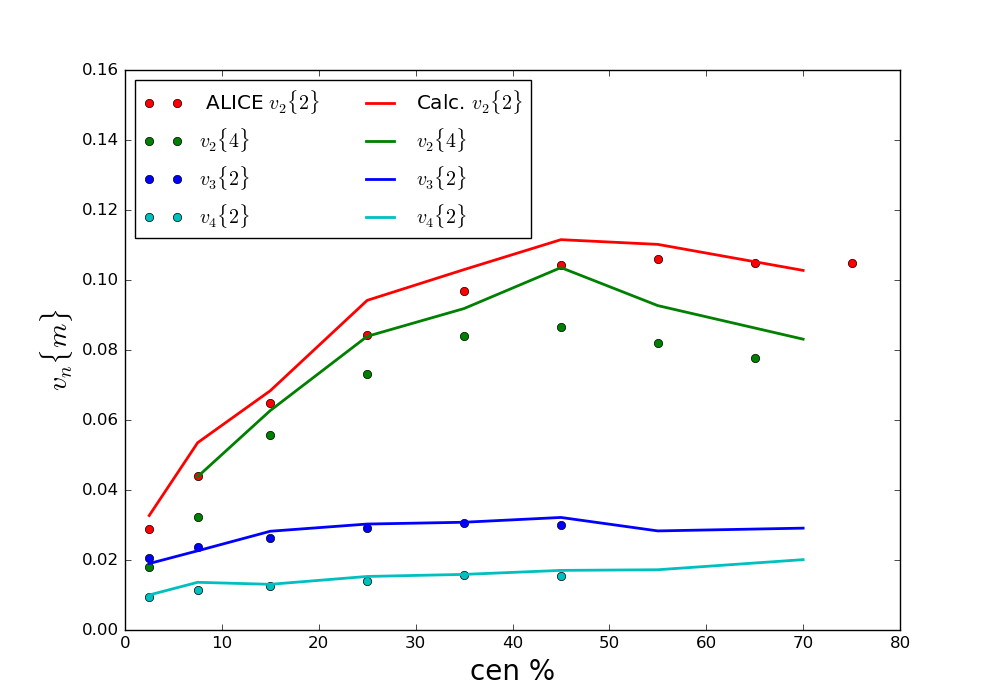
\includegraphics[width=\columnwidth]{pics/new-PbPb-vnm-p1.png}	
	\caption{Centrality dependence of anisotropic flow $v_n\{m\}$ of PbPb collision at $\sqrt{s} = 2.76$ TeV.}
  	\label{PbPb-vn-calc}
	\end{figure}
	
	\begin{figure}
  	\centering
	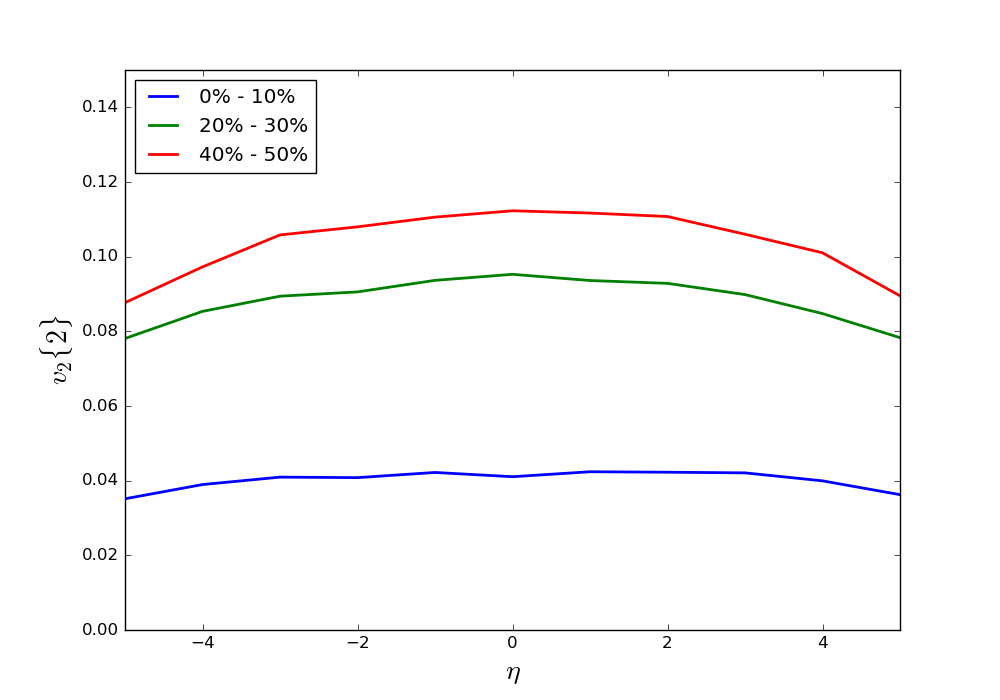
\includegraphics[width=\columnwidth]{pics/new-PbPb-vnm-eta-p1.png}
	\caption{Pseudo-rapidity dependence of anisotropic flow $v_2\{2\}$ of PbPb collision at $\sqrt{s} = 2.76$ TeV.}
  	\label{PbPb-vn-eta-calc}
	\end{figure}
	
	\begin{figure}
  	\centering
	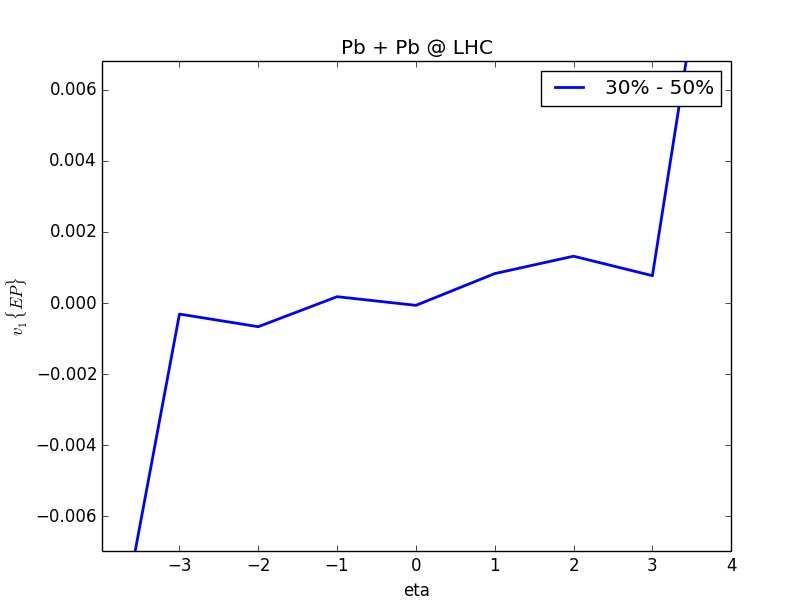
\includegraphics[width=\columnwidth]{pics/RUN-1-PbPb-v1-eta.png}
	\caption{Pseudo-rapidity dependence of average transverse momentum $\langle\langle \mathbf{p}_T\cdot \hat{b}/p_T\rangle\rangle$ as an estimation of directed flow of PbPb collision at $\sqrt{s} = 2.76$ TeV.}
  	\label{RUN-1-PbPb-v1-eta}
	\end{figure}
	
	These results by no means represent a best fit to experiment, but just demonstrate that 3d extended TRENTo initial condition combined with state-of-the-art hybrid model is able to capture the qualitative features of a variety of experimental observables -- especially those with pseudo-rapidity dependence.
	The model has the potential to describe the experimental data quantitatively and more importantly, constrains our knowledge of initial state and QGP transport properties simultaneously through model-to-data comparison.
	
\section{Summary and Outlooks}
	In summary, we extended the phenomenological initial condition model TRENTo for relativistic heavy ion collision from two to three dimensions. 	
	The parametrization is simple and flexible to investigate different longitudinal entropy deposition schemes. 	
	Using Bayesian analysis, initial condition model parameters are constrained by experimental observables that are not sensitive to dynamics. 	
	The present entropy deposition scheme very well describes the observed charged particle pseudo-rapidity distribution of both symmetric and asymmetric collision at LHC energies.
	We obtained the posterior probability distribution of model parameters, which shows that longitudinal entropy deposition favours a slightly skewed profile centred around the center of mass rapidity of local target and projectile densities.

	We calculated more observables after full time evolution, especially those with longitudinal dependence, and showed that the model captures the qualitative feature of experimental data.

	A model-to-data comparison with an enlarged set of observables will put much stronger constraints on initial condition models and at the same time improve our knowledge of QGP shear and bulk viscosity. 

	Of course, as stated previously, a 3+1 D model is computationally intense. So we will next focus on improving the efficiency of the calculation. This could include code optimization, reducing model complexity by maximizing model likelihood and feeding our present result as priori for the next, more complicated statistical analysis.

\section{Acknowledgements}

% If in two-column mode, this environment will change to single-column
% format so that long equations can be displayed. Use
% sparingly.
%\begin{widetext}
% put long equation here
%\end{widetext}

% figures should be put into the text as floats.
% Use the graphics or graphicx packages (distributed with LaTeX2e)
% and the \includegraphics macro defined in those packages.
% See the LaTeX Graphics Companion by Michel Goosens, Sebastian Rahtz,
% and Frank Mittelbach for instance.
%
% Here is an example of the general form of a figure:
% Fill in the caption in the braces of the \caption{} command. Put the label
% that you will use with \ref{} command in the braces of the \label{} command.
% Use the figure* environment if the figure should span across the
% entire page. There is no need to do explicit centering.

% \begin{figure}
% \includegraphics{}%
% \caption{\label{}}
% \end{figure}

% Surround figure environment with turnpage environment for landscape
% figure
% \begin{turnpage}
% \begin{figure}
% \includegraphics{}%
% \caption{\label{}}
% \end{figure}
% \end{turnpage}

% tables should appear as floats within the text
%
% Here is an example of the general form of a table:
% Fill in the caption in the braces of the \caption{} command. Put the label
% that you will use with \ref{} command in the braces of the \label{} command.
% Insert the column specifiers (l, r, c, d, etc.) in the empty braces of the
% \begin{tabular}{} command.
% The ruledtabular enviroment adds doubled rules to table and sets a
% reasonable default table settings.
% Use the table* environment to get a full-width table in two-column
% Add \usepackage{longtable} and the longtable (or longtable*}
% environment for nicely formatted long tables. Or use the the [H]
% placement option to break a long table (with less control than 
% in longtable).
% \begin{table}%[H] add [H] placement to break table across pages
% \caption{\label{}}
% \begin{ruledtabular}
% \begin{tabular}{}
% Lines of table here ending with \\
% \end{tabular}
% \end{ruledtabular}
% \end{table} 

% Surround table environment with turnpage environment for landscape
% table
% \begin{turnpage}
% \begin{table}
% \caption{\label{}} 
% \begin{ruledtabular}
% \begin{tabular}{}
% \end{tabular}
% \end{ruledtabular}
% \end{table}
% \end{turnpage}

% Specify following sections are appendices. Use \appendix* if there
% only one appendix.
%\appendix
%\section{}

% If you have acknowledgments, this puts in the proper section head.
%\begin{acknowledgments}
% put your acknowledgments here.
%\end{acknowledgments}

% Create the reference section using BibTeX: 
\bibliography{report2Notes} 

\end{document}
%
% ****** End of file apstemplate.tex ******

